\documentclass[12pt,a4paper,article,english,firamath]{nsi}
\pagestyle{empty}
\setfontfamily{\brettley}{Cursive standard}[Scale=1.5]
\begin{document}
\titre{Find your figure}
\classe{Euro 1\ere}
\maketitle

\subsection*{Description 4}
{\brettley 

Draw a line segment and a circle passing through its endpoints, whose center is the line segment's midpoint.
Draw two other line segments passing through the endpoints of the first one, perpendicularly to it. The new segments should have the same length as the initial one and be on the same side of it. Join the second endpoints of the two new segments. Draw a line joining two of the four points, diagonally.}\\[1em]

\begin{tikzpicture}
    \draw[lightgray](0,0)--(\linewidth,0);
\end{tikzpicture}


\subsection*{Figure 5}
\begin{center}
    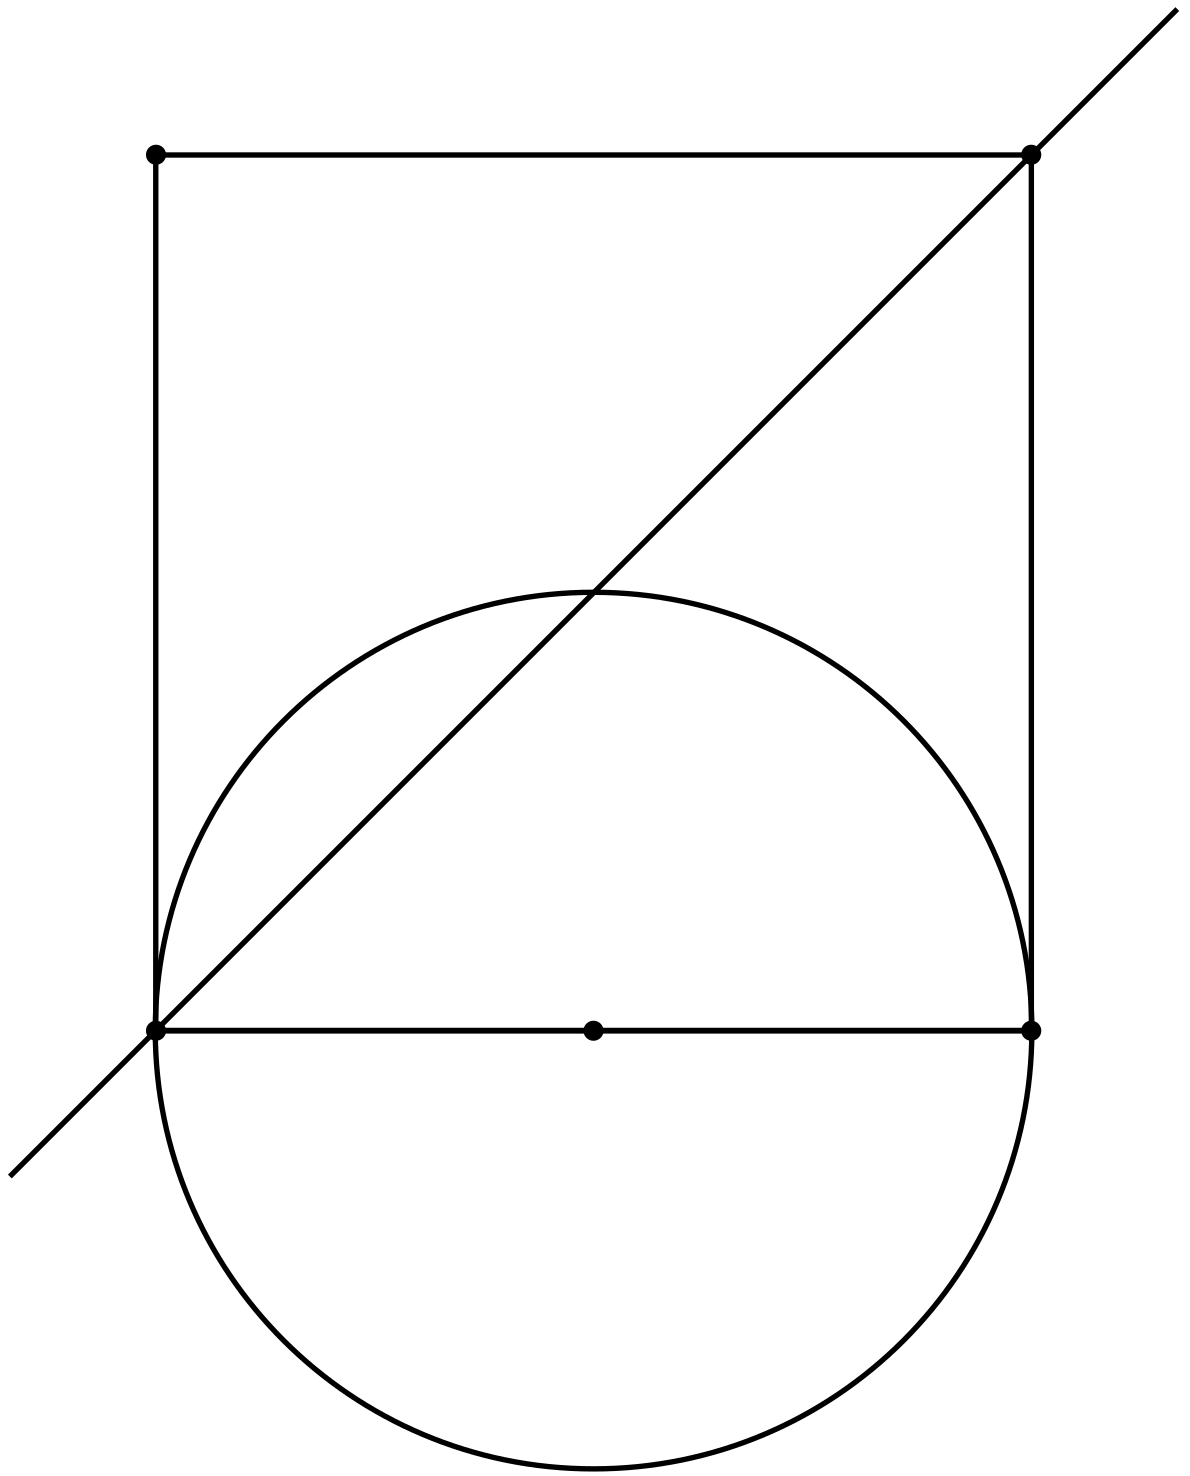
\includegraphics[height=12cm]{img/fig04.png}
\end{center}
\end{document}